\section{Анализ предметной области ассистентов организации времени}
\label{sec:analysis}


В данном разделе проводится комплексный анализ предметной области разрабатываемого проекта, по итогам которого будет сформирован исчерпывающий перечень требований к программной системе для ее последующего архитектурного проектирования. Для полноценного исследования требуется дать точную характеристику рассматриваемой сферы. Выявление ключевых понятий и принципов позволит логично перейти к глубокому анализу существующей проблематики и критическому обзору релевантных решений.

Для обоснования актуальности и научной новизны работы определены следующие задачи исследования предметной области:

\begin{enumerate}[label=\arabic*]
    \item Характеристика предметной области, включающая определение ключевых понятий и описание базовых принципов проведения исследования.

    \item Раскрытие проблематики организации времени в академической среде. Выявление основных барьеров, препятствующих эффективному процессу обучения.

    \item Критический анализ существующих аналогов для определения инструментария, применяемого на сегодняшний день. Сравнение будет производиться по заранее установленным критериям для выявления достоинств и недостатков каждого решения.

    \item Сравнение современных технологических подходов к разработке. Особое внимание уделяется диалоговым агентным системам на базе больших языковых моделей (LLM), способным к автономной декомпозиции задач, распределению учебной нагрузки и бесшовной интеграции с календарем пользователя.

\end{enumerate}

В результате выполнения поставленных задач будет составлен формализованный список функциональных и нефункциональных требований к персональному ассистенту, что позволит грамотно спроектировать и реализовать программную систему целиком.


\subsection{Характеристика предметной области}

Для всестороннего понимания контекста разрабатываемой системы необходимо четко очертить границы предметной области, которые детерминируются темой дипломного проекта и спецификой его целевой аудитории. Характеристика предметной области включает в себя выявление и определение ключевых терминов, а также установление логических взаимосвязей между ними. На основе данного понятийного аппарата будут сформулированы базовые принципы исследования. Эти принципы позволят системно проанализировать проблематику, обосновать актуальность предлагаемого решения и выбрать наиболее оптимальные технологические подходы к его реализации.


% \stepcounter{subsubsection}
% \subsubsection*{\thesubsubsection\space Описание ключевых понятий предметной области}
\subsubsection{Описание ключевых понятий предметной области}

Предметная область исследования ограничивается спецификой цифрового ассистирования в контексте образовательного процесса. Базовым понятием в данном случае выступает \textbf{организация времени (time-management)}. В целом, единого академического определения данного понятия нет, однако на основе крупного метаанализа работ, посвященных вопросу управления временем \cite{Time-managemnet_review}, предлагается определить его как ``совокупность форм поведения, направленных на достижение эффективного использования времени при выполнении определенных целенаправленных действий''. Авторы выделяют несколько ключевых аспектов организации времени:   
\begin{enumerate}[label=\arabic*]
    \item Оценка времени подразумевает осознание текущего момента и временной перспективы. Оценка строится на основе самоанализа того, как именно расходуется время. Это также включает рефлексию собственных субъективных установок и когнитивного восприятия времени. Это позволяет объективно оценить выполнимый объём задач на текущий отрезок времени.
    \item Планирование включает целеполагание, планирование конкретных задач и их приоритизацию. К планированию также относится составление списков дел и группировка задач. За счёт такой структуризации появляется возможность эффективно спланировать временные ресурсы.
    \item Отслеживание расхода времени также способствует его рациональному использованию, но в динамике. По ходу выполнения задач, человек анализирует темпы их выполнения и в дальнейшем корректирует планы.
\end{enumerate}

Таким образом, формирование контролируемой среды для достижения целей опирается на описанную триаду поведенческих паттернов. В рамках данного исследования именно эти структурные компоненты саморегуляции выступят методологической основой для проектирования логики принятия решений разрабатываемого интеллектуального ассистента. 

В контексте управления и организации времени критичным является наличие соответствующих навыков у субъекта. Ведь исторически принципы менеджмента развивались для управления сложными производственными и бизнес-процессами, поскольку любая многокомпонентная деятельность требует выделения отдельного ресурса на координацию и контроль. 

В современной образовательной парадигме этот принцип масштабируется до индивидуального уровня: обучение приобретает черты долгосрочной проектной деятельности, где студент выступает в роли менеджера собственного образовательного маршрута. Это особенно актуально для инженерных специальностей, где преобладают такие формы работ, как: лабораторные практикумы, курсовые и дипломные проекты, ориентированные на продолжительную практическую работу, требующую комплексного подхода к решению задач. Это порождает потребность в развитии навыков персонального управления и организации времени.

На практике управленческая деятельность требует значительных когнитивных ресурсов. Процессы планирования, оценки масштабов задачи и мониторинга расходуют те же ментальные резервы, что и непосредственно учебная деятельность. И зачастую, именно отсутствие навыков планирования и декомпозиции целей приводит часто к неверной субъективной оценке времени, которое требуется уделить задаче. Соответственно, возникает \textbf{прокрастинация}. Это иррациональная привычка добровольно откладывать задачи, несмотря на осознание того, что это приведёт к негативным последствиям \cite{Procrastination_Peers}. Отдельные исследования были посвящены прокрастинации в учебной среде \cite{Schouwenburg2004}, и на сегодняшний день выделяют следующие причины подобного поведения:

\begin{itemize}
    \item эмоционально-поведенческие включают страх неудачи, перфекционизм, способность удерживать фокус внимания;
    \item когнитивные факторы включают отсутствие навыков планирования постановку нечётких целей;
    \item мотивационные - то есть личная мотивация к учёбе;
    \item личностные качества, которые делают человека склонным к прокрастинации;
\end{itemize}

Если мотивационные и личностные факторы лежат в плоскости психологии, то когнитивные причины прокрастинации (отсутствие плана, неясность шагов) могут быть устранены техническими средствами. Планирование и декомпозиция задач — это процессы, поддающиеся алгоритмизации и формализации. Современные прикладные программы способны взять на себя выполнение этих формализуемых когнитивных задач, выступая в роли внешней системы управления и контроля.

Следствием необходимости преодоления прокрастинации и структурирования учебной нагрузки является высокая потребность в специализированных программных инструментах. К таким базовым инструментам исторически относятся цифровые календари для визуализации расписания, трекеры задач для мониторинга прогресса, а также системы внешней мотивации и уведомлений. Однако разрозненность этих средств и необходимость их ручного заполнения создают дополнительную когнитивную нагрузку на обучающегося.

Это противоречие приводит к возникновению концепции \textbf{интеллектуального персонального ассистента} — программной системы, способной не просто агрегировать функционал планировщика, но и выступать в роли активного наставника. В рамках данной работы персональный ассистент рассматривается как диалоговая агентная система, которая берет на себя рутину по декомпозиции крупных учебных целей (разбиению их на атомарные, выполнимые шаги) и формированию оптимального графика их достижения, динамически адаптируясь под индивидуальные ритмы и занятость пользователя.


% \stepcounter{subsubsection}
% \subsubsection*{\thesubsubsection\space Принципы исследования предметной области}
\subsubsection{Принципы исследования предметной области}

Для обеспечения научной обоснованности и практической ценности разрабатываемого продукта исследование и проектирование в рамках предметной области опираются на ряд фундаментальных принципов.

С точки зрения научно-исследовательского подхода, первостепенным является \textbf{принцип системности}. Он предписывает рассматривать процесс организации учебного времени не изолированно, а как сложную динамическую систему, зависящую от множества пересекающихся факторов: жесткого расписания занятий в учебном заведении, сроков сдачи работ, сторонней занятости студента и его индивидуальной утомляемости. Также применяется \textbf{принцип объективности данных}, требующий опираться на достоверные показатели активности пользователя (например, посредством интеграции с системами контроля версий кода или университетскими образовательными платформами) для оценки реального прогресса, минимизируя зависимость от субъективного ручного ввода информации.

С позиции программной инженерии и проектирования архитектуры, разработка руководствуется \textbf{принципом приоритета интеллектуальных технологий}. Это подразумевает использование передовых достижений в области искусственного интеллекта, в частности, интеграцию больших языковых моделей в качестве когнитивного ядра (агента). Агент должен быть способен вести диалог на естественном языке и осуществлять логический вывод для интеллектуального разбиения задач.

Кроме того, программная реализация должна подчиняться общепринятым архитектурным практикам: \textbf{принципу модульности и масштабируемости}, что позволит в будущем легко интегрировать новые источники данных или сторонние календари. Критически важным для пользовательского опыта является \textbf{принцип транзакционности изменений} — любые модификации личного расписания пользователя, предлагаемые ИИ-ассистентом, должны носить характер «черновика» (проекта расписания) с обязательной возможностью предпросмотра, подтверждения или отката до предыдущего состояния. Это гарантирует безопасность персональных данных пользователя и исключает внесение хаоса в уже устоявшийся график.


\subsection{Проблематика организации времени}

В ходе обзора предметной области исследования было установлено, что потребность в средствах организации времени тесно связана с дефицитом навыков планирования, что закономерно приводит к такому явлению, как прокрастинация. Чтобы определить эффективные пути помощи пользователю в преодолении этого состояния, необходимо рассмотреть природу данного феномена, выявить его основные причины и проанализировать существующие программные решения в этой области. 

% \stepcounter{subsubsection}
% \subsubsection*{\thesubsubsection\space Феномен академической прокрастинации в условиях слабой структурированности учебного процесса}
\subsubsection{Феномен академической прокрастинации в условиях слабой структурированности учебного процесса}

Рассматривая прокрастинацию, следует отказаться от распространенного бытового заблуждения, согласно которому она является исключительно следствием индивидуальной лени. Наличие обширной базы научных исследований доказывает обратное и свидетельствует о массовом характере проблемы, порождающем устойчивый спрос на разработку специфических методов ее преодоления.

Так, нейропсихологическое исследование, проведенное среди студентов высших учебных заведений \cite{Rabin2011}, выявило конкретную когнитивную составляющую этого процесса. Авторы напрямую связывают склонность к прокрастинации со слабым развитием исполнительных функций префронтальной коры мозга, отвечающих за инициацию, планирование и организацию деятельности. Эти данные свидетельствуют о том, что прокрастинация обусловлена объективным дефицитом когнитивных механизмов, который, тем не менее, поддается успешной компенсации при интеграции внешних организационных стратегий и инструментов.

В связи с этим в современной педагогике прокрастинация рассматривается как фундаментальное нарушение процессов саморегуляции обучения (self-regulated learning). Как отмечает Б. Зиммерман, основным фактором, обнажающим этот дефицит, становится резкое изменение специфики учебной среды при переходе на более высокие ступени образования \cite{Zimmerman2002}. В отличие от школьной системы, где преобладает жесткий внешний контроль и короткие итерации оценивания (ежедневные домашние задания), академическая среда вуза характеризуется слабой структурированностью процессов и высокой потребностью в автономии. 

Обучающийся сталкивается с объемными, долгосрочными проектами (курсовые работы, комплексные лабораторные практикумы), дедлайны по которым значительно отдалены во времени. Отсутствие регулярного промежуточного контроля перекладывает всю когнитивную нагрузку по целеполаганию, оценке времени и распределению усилий непосредственно на студента. Исследования показывают, что когда когнитивная сложность самостоятельного планирования глобальной задачи превышает текущие возможности исполнительных функций обучающегося, возникает защитная реакция психики — избегание, выражающееся в иррациональном откладывании действий. 

Таким образом, для преодоления академической прокрастинации необходимо искусственно структурировать среду, делегируя процессы алгоритмической декомпозиции, планирования и микро-контроля специализированным программным инструментам.


% \stepcounter{subsubsection}
% \subsubsection*{\thesubsubsection\space Проблематика концентрации внимания на долгосрочной задаче}
\subsubsection{Проблематика концентрации внимания на долгосрочной задаче}

Структурирование задачи решает проблему «холодного старта», однако длительные академические проекты характеризуются естественным спадом мотивации, что требует механизмов постоянного удержания фокуса внимания. Для повышения вовлеченности (compliance) пользователей в современных программных решениях активно применяются методы поведенческой экономики и геймификации, опирающиеся на фундаментальные когнитивные особенности человеческой психики. Рассмотрим несколько актуальных теорий и методологий, которые предлагают решение проблемы удержания внимания. 

Основополагающим подходом к формированию привычек является теория подталкивания (Nudge theory), предложенная Р. Талером и К. Санстейном \cite{Thaler2008}. Авторы обосновывают необходимость создания такой «архитектуры выбора», при которой оптимальное решение становится для пользователя путем наименьшего сопротивления, не требуя при этом жесткого внешнего принуждения. Это наблюдение говорит о важности такого функционала, как уведомления пользователя, а также о необходимости проактивного поведение ассистента: например предложение ассистентом готового расписания на день, или ненавязчивые уведомления о сроках задачи. 


Важным аспектом удержания внимания является стимуляция потребности закрыть поставленную задачу. Экспериментально доказано, что прерванные или незавершенные действия вызывают психологическое напряжение (дискомфорт) и запоминаются значительно лучше, чем завершенные — данный феномен известен как эффект Зейгарник \cite{Zeigarnik1927}. В контексте цифрового обучения, как отмечают современные исследователи, визуализация этого дискомфорта с последующим его разрешением активно стимулирует дофаминовую систему поощрения \cite{Syndell2020}. В контексте разработки цифрового помощника, можно сделать вывод, что абстрактная и долгосрочная цель («сдать сессию») должна быть конвертирована в серию осязаемых короткорсочных целей (подобно так называемым ``спринтам'' в методологии управления ``Scrum'' \cite{Stahl1990}). Использование диаграмм Ганта, заполняющихся шкал прогресса (progress bars) и трекеров привычек визуализирует эффект Зейгарник. Каждое нажатие чекбокса выполненной подзадачи снимает когнитивное напряжение и обеспечивает быстрый дофаминовый отклик, формируя петлю положительной обратной связи. 


Для поддержания регулярной ежедневной активности наиболее эффективным механизмом является эксплуатация когнитивного искажения «неприятия потери» (loss aversion). Согласно фундаментальным выводам теории перспектив Д. Канемана и А. Тверски \cite{Kahneman1979}, разочарование от потери накопленного ресурса субъективно переживается индивидом в два раза острее, чем радость от получения эквивалентного приобретения. Таким образом, в архитектуру ассистента целесообразно внедрить систему счетчика дней непрерывной учебной активности, успешно применяемую в платформах вроде Duolingo~\cite{duolingo}. Накапливая визуальный прогресс непрерывной работы, пользователь попадает в условия, когда прервать цепочку дней (потерять статус) становится психологически тяжелее, чем выполнить минимально требуемую учебную задачу.



\subsection{Анализ аналогов разрабатываемой системы}
% \stepcounter{subsubsection}

В данном разделе будет проведён анализ существующих решений в области организации времени и управления задачами.
Целью этого анализа является выявление функционала этих решений, а также определение возможностей для улучшения и инноваций в нашем проекте. Также рассмотрим,
как эти системы справляются с проблемами, описанными в предыдущем разделе, и какие методы они используют для повышения вовлеченности пользователей.


% \subsubsection*{\thesubsubsection\space Duolingo: геймификация и удержание пользователей в образовательных приложениях}
\subsubsection{Duolingo. Геймификация и удержание пользователей в образовательных приложениях}

Duolingo~\cite{duolingo} представляет собой интерактивную образовательную платформу, первоначально ориентированную на изучение иностранных языков. Основным предназначением системы является демократизация образовательного процесса и трансформация рутинного заучивания в увлекательный процесс. Целевая аудитория приложения максимально широка и охватывает пользователей всех возрастов, занимающихся самообразованием. В контексте данного исследования платформа представляет особый интерес не как инструмент прямого планирования, а как эталонная реализация механизмов удержания внимания (комплаенса) и мотивации при работе с долгосрочными целями.

\begin{figure}[H]
\centering
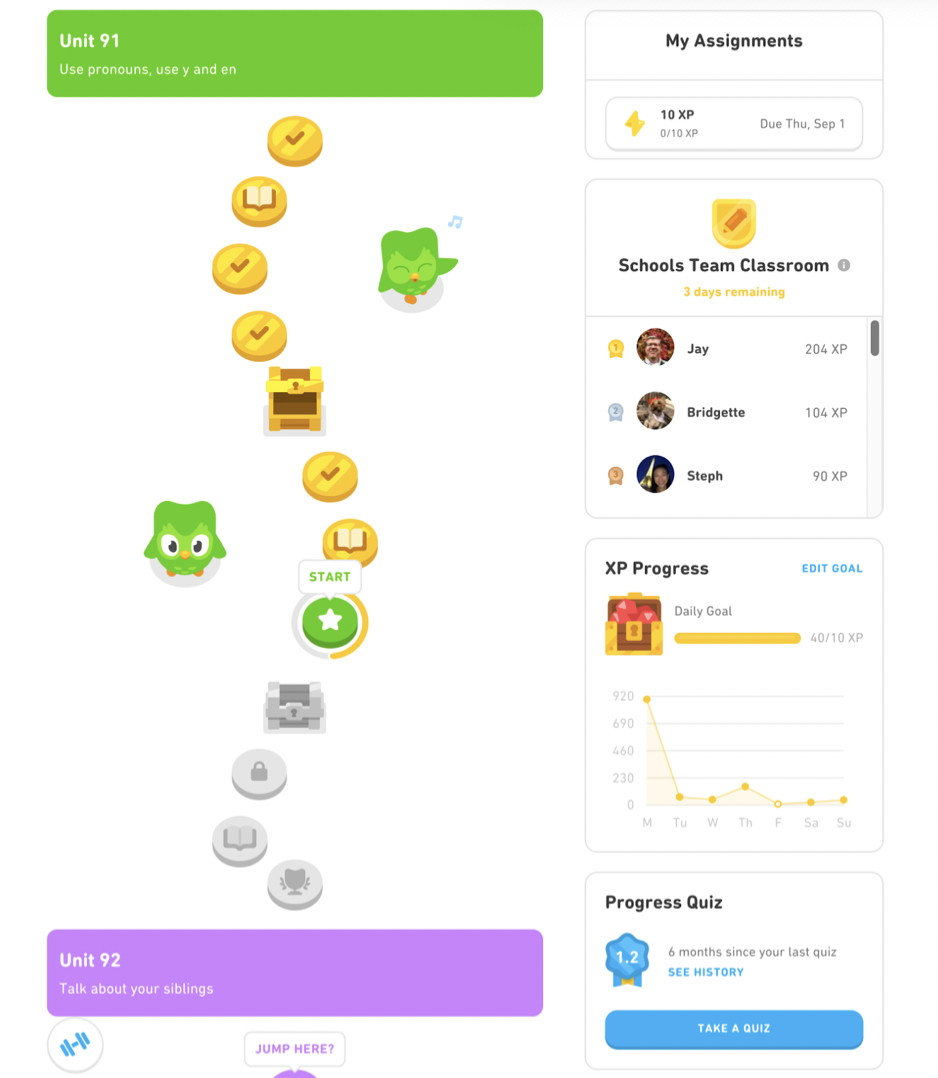
\includegraphics[width=0.7\linewidth]{picture/duolingo.png}
\caption{Интерфейс приложения Duolingo}
\label{fig:duolingo}
\end{figure}

Как видно на рисунке \ref{fig:duolingo}, функциональные возможности платформы строго подчинены принципам поведенческой экономики:

\begin{enumerate}[label=\arabic*]
\item Счетчик дней подряд, в которые пользователь выполнял хотя бы минимальную норму заданий. Механизм эксплуатирует когнитивное искажение неприятия потери, стимулируя пользователя возвращаться в приложение ежедневно.
\item Глобальная цель (выучить язык) жестко декомпозирована на атомарные уроки длительностью 3-5 минут, что радикально снижает когнитивный барьер для начала занятий (решение проблемы «холодного старта»).
\item Использование шкал прогресса, очков опыта (XP) и соревновательных лиг, обеспечивающих быструю дофаминовую обратную связь за каждое совершенное действие.
\item Адаптивная система push-уведомлений, напоминающая о необходимости выполнить урок до истечения суток, выступающая в роли внешнего триггера для формирования привычки.
\end{enumerate}

% \stepcounter{subsubsection}
% \subsubsection*{\thesubsubsection\space Akiflow: интеграция с календарями и управление задачами для повышения продуктивности}
\subsubsection{Akiflow. Интеграция с календарями и управление задачами для повышения продуктивности}

Akiflow~\cite{akiflow} позиционируется как централизованный программный хаб для профессионального тайм-блокинга (метода управления временем, при котором под каждую задачу выделяется фиксированный слот в календаре). Основная цель приложения — агрегация всех дел пользователя в едином пространстве для предотвращения переключений между разными контекстами. Целевая аудитория системы включает профессионалов, менеджеров и предпринимателей, чья деятельность связана с большим объемом операционных задач, распределенных по различным корпоративным сервисам.

\begin{figure}[H]
\centering
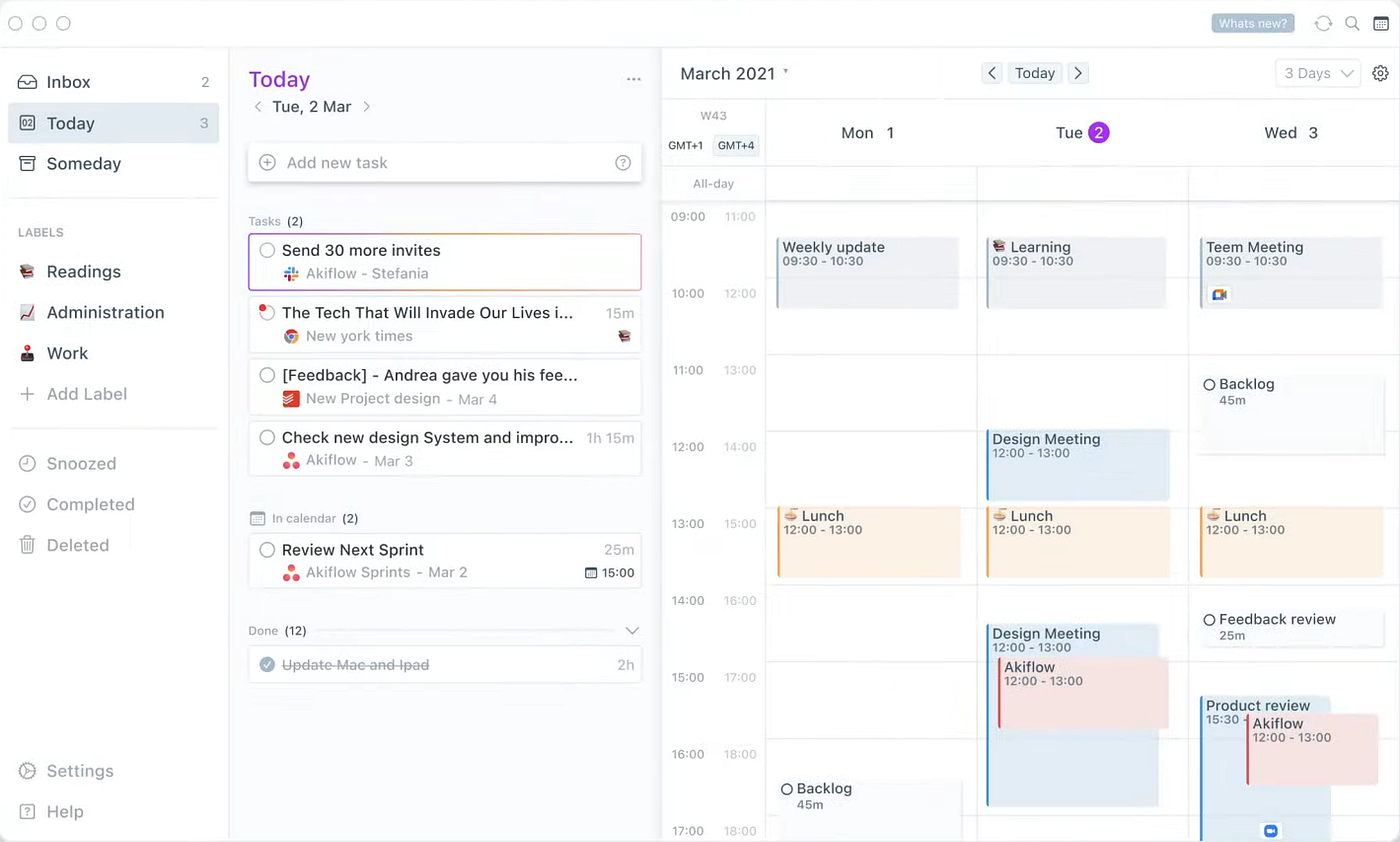
\includegraphics[width=0.9\linewidth]{picture/akiflow.png}
\caption{Интерфейс тайм-блокера akiflow}
\label{fig:akiflow}
\end{figure}

Как показано на рисунке \ref{fig:akiflow}, система предлагает следующий функционал:

\begin{enumerate}[label=\arabic*]
\item Автоматический сбор задач из внешних экосистем (электронная почта, мессенджеры, трекеры задач) в один список.
\item Инструментарий для ручного перетаскивания задач из списка в календарную сетку.
\item Возможность быстрого создания задач путем текстового описания (например, установление даты и дедлайна через текст).
\item Встроенные сценарии утреннего планирования и вечернего подведения итогов, заставляющие пользователя регулярно пересматривать свой список дел.
\item Автоматическая категоризация задач и базовые предложения оптимального времени для их выполнения, однако система остается реактивной — она управляет уже существующими задачами, но не генерирует алгоритм их выполнения с нуля.
\end{enumerate}

% \stepcounter{subsubsection}
% \subsubsection*{\thesubsubsection\space Reclaim: автоматическое планирование задач и управление временем для оптимизации рабочего процесса}
\subsubsection{Reclaim. Автоматическое планирование задач и управление временем для оптимизации рабочего процесса}

Reclaim (Reclaim.ai)~\cite{reclaim} представляет собой интеллектуальную надстройку над цифровыми календарями, специализирующуюся на умном блокировании времени и защите фокусных часов. Главное предназначение системы — динамическая оптимизация расписания в условиях постоянно меняющихся приоритетов и входящих встреч. Целевой аудиторией являются занятые специалисты и команды, испытывающие проблемы с балансировкой между проектной работой и рутинными обязанностями.

\begin{figure}[H]
\centering
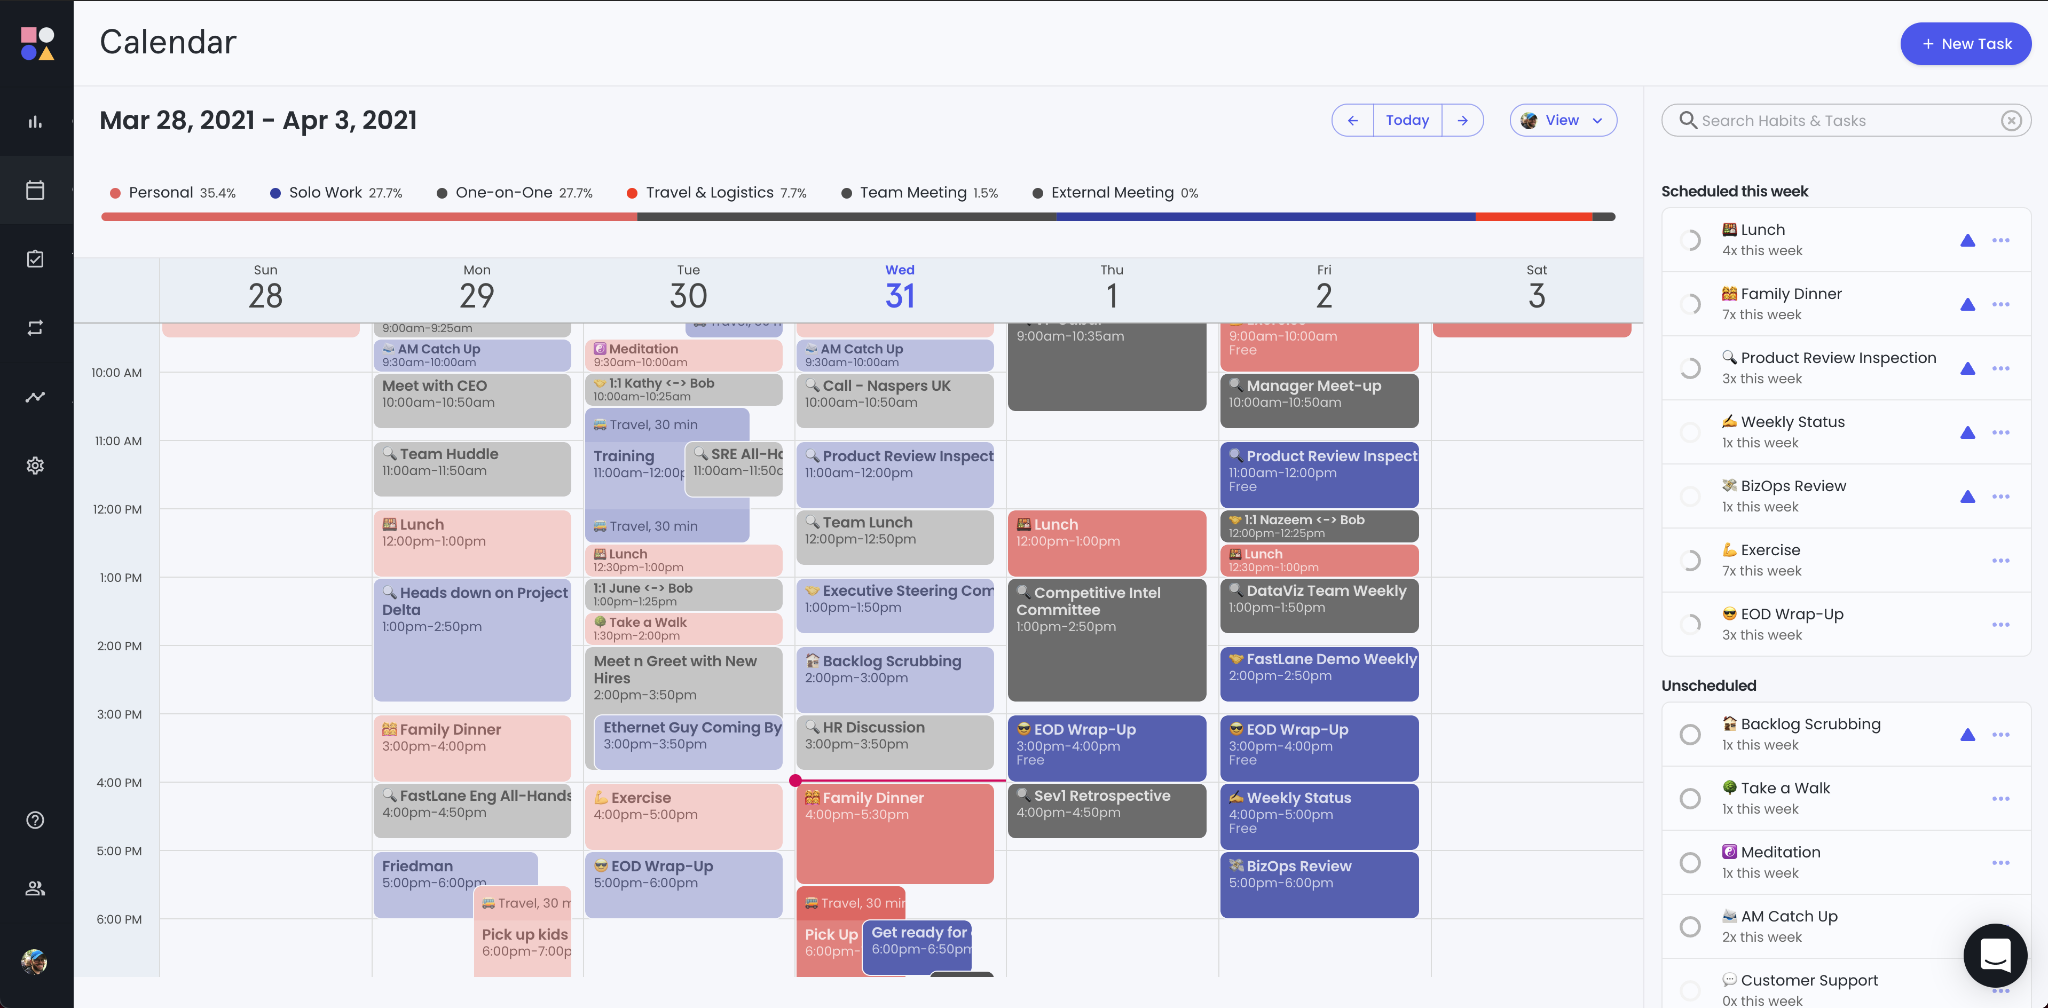
\includegraphics[width=0.9\linewidth]{picture/reclaim.png}
\caption{Интерфейс планера Reclaim}
\label{fig:reclaim}
\end{figure}

Интерфейс, представленный на рисунке \ref{fig:reclaim}, отражает фокус системы на автоматизации:

\begin{enumerate}[label=\arabic*]
\item Алгоритм самостоятельно находит окна в расписании для выполнения задач из списка. Если появляется срочная встреча, система автоматически перемещает запланированные задачи на другие свободные слоты без ручного вмешательства пользователя.
\item Отдельный модуль для защиты времени на регулярные, но гибкие активности (например, чтение, тренировки, обед), которые система размещает в течение дня или недели.
\item Автоматическое добавление перерывов между плотно идущими событиями для снижения когнитивной усталости.
\item Предоставление детальных отчетов о том, на какие категории деятельности (встречи, глубокая работа, личные дела) был потрачен временной ресурс.
\end{enumerate}

% \stepcounter{subsubsection}
% \subsubsection*{\thesubsubsection\space Google Workspace: инструменты для организации времени и совместной работы в образовательных учреждениях}
\subsubsection{Google Workspace. Инструменты для организации времени и совместной работы в образовательных учреждениях}

Google Workspace~\cite{google_workspace} — это комплексная облачная экосистема корпоративного уровня, включающая в себя инструменты для создания документов, коммуникации и планирования. В контексте тайм-менеджмента ядром системы выступает плотная интеграция Google Calendar, Google Tasks и Gmail. Целевая аудитория варьируется от индивидуальных пользователей до крупнейших корпораций и образовательных учреждений, для которых система выступает базовой инфраструктурой.

\begin{figure}[H]
\centering
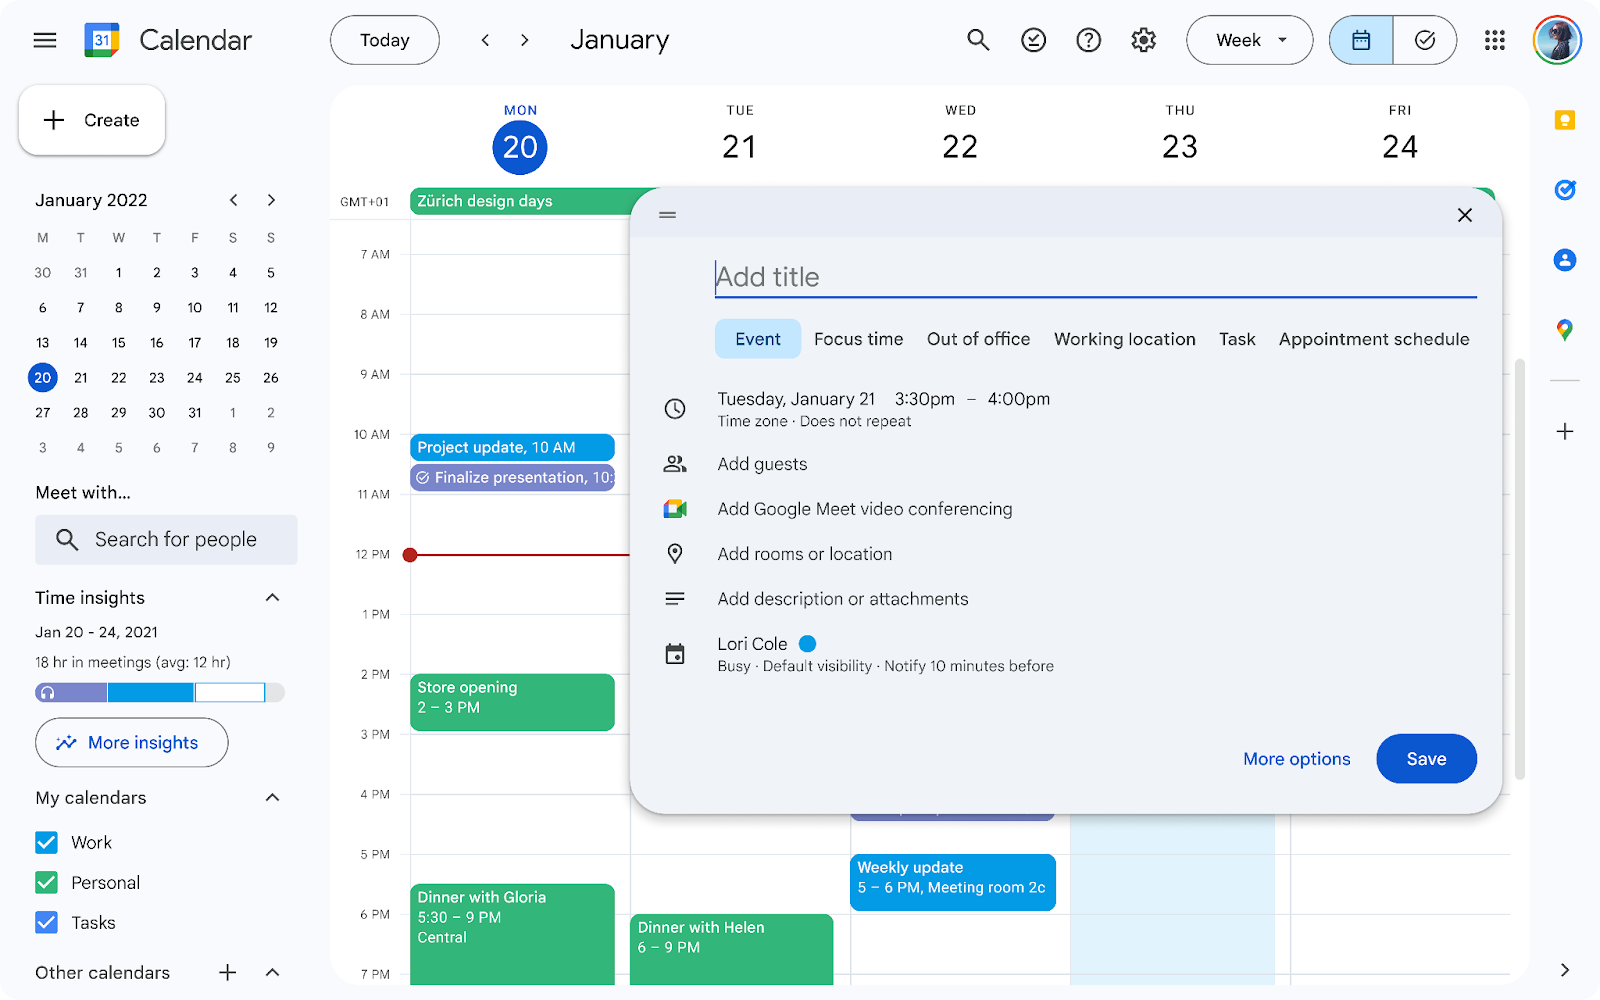
\includegraphics[width=0.9\linewidth]{picture/google.png}
\caption{Интерфейс системы google workspace}
\label{fig:google}
\end{figure}

Как иллюстрирует рисунок \ref{fig:google}, инструментарий системы носит ярко выраженный универсальный характер:

\begin{enumerate}[label=\arabic*]
\item Бесшовное преобразование входящих писем или комментариев в документах в задачи с их последующим отображением в календаре.
\item Возможность наложения календарей нескольких пользователей, автоматический поиск свободных слотов для групповых встреч.
\item Использование генеративного искусственного интеллекта для анализа контекста писем, составления расписания встреч и извлечения сущностей из документов.
\item Система предоставляет фундаментальный инструментарий горизонтального планирования, однако лишена вертикально-ориентированных функций для академической среды (нет встроенных механизмов декомпозиции образовательных целей или геймифицированного удержания фокуса).
\end{enumerate}

% \stepcounter{subsubsection}
% \subsubsection*{\thesubsubsection\space Moodle: платформа для управления обучением и организации учебного процесса в академической среде}
\subsubsection{Moodle. Платформа для управления обучением и организации учебного процесса в академической среде}

Moodle~\cite{moodle} является классическим примером системы управления обучением (Learning Management System, LMS). Основная цель платформы — предоставление цифровой среды для администрирования учебных курсов, распространения образовательных материалов и оценки знаний. Целевой аудиторией выступают образовательные учреждения (ВУЗы, школы), преподаватели и студенты.

\begin{figure}[H]
\centering
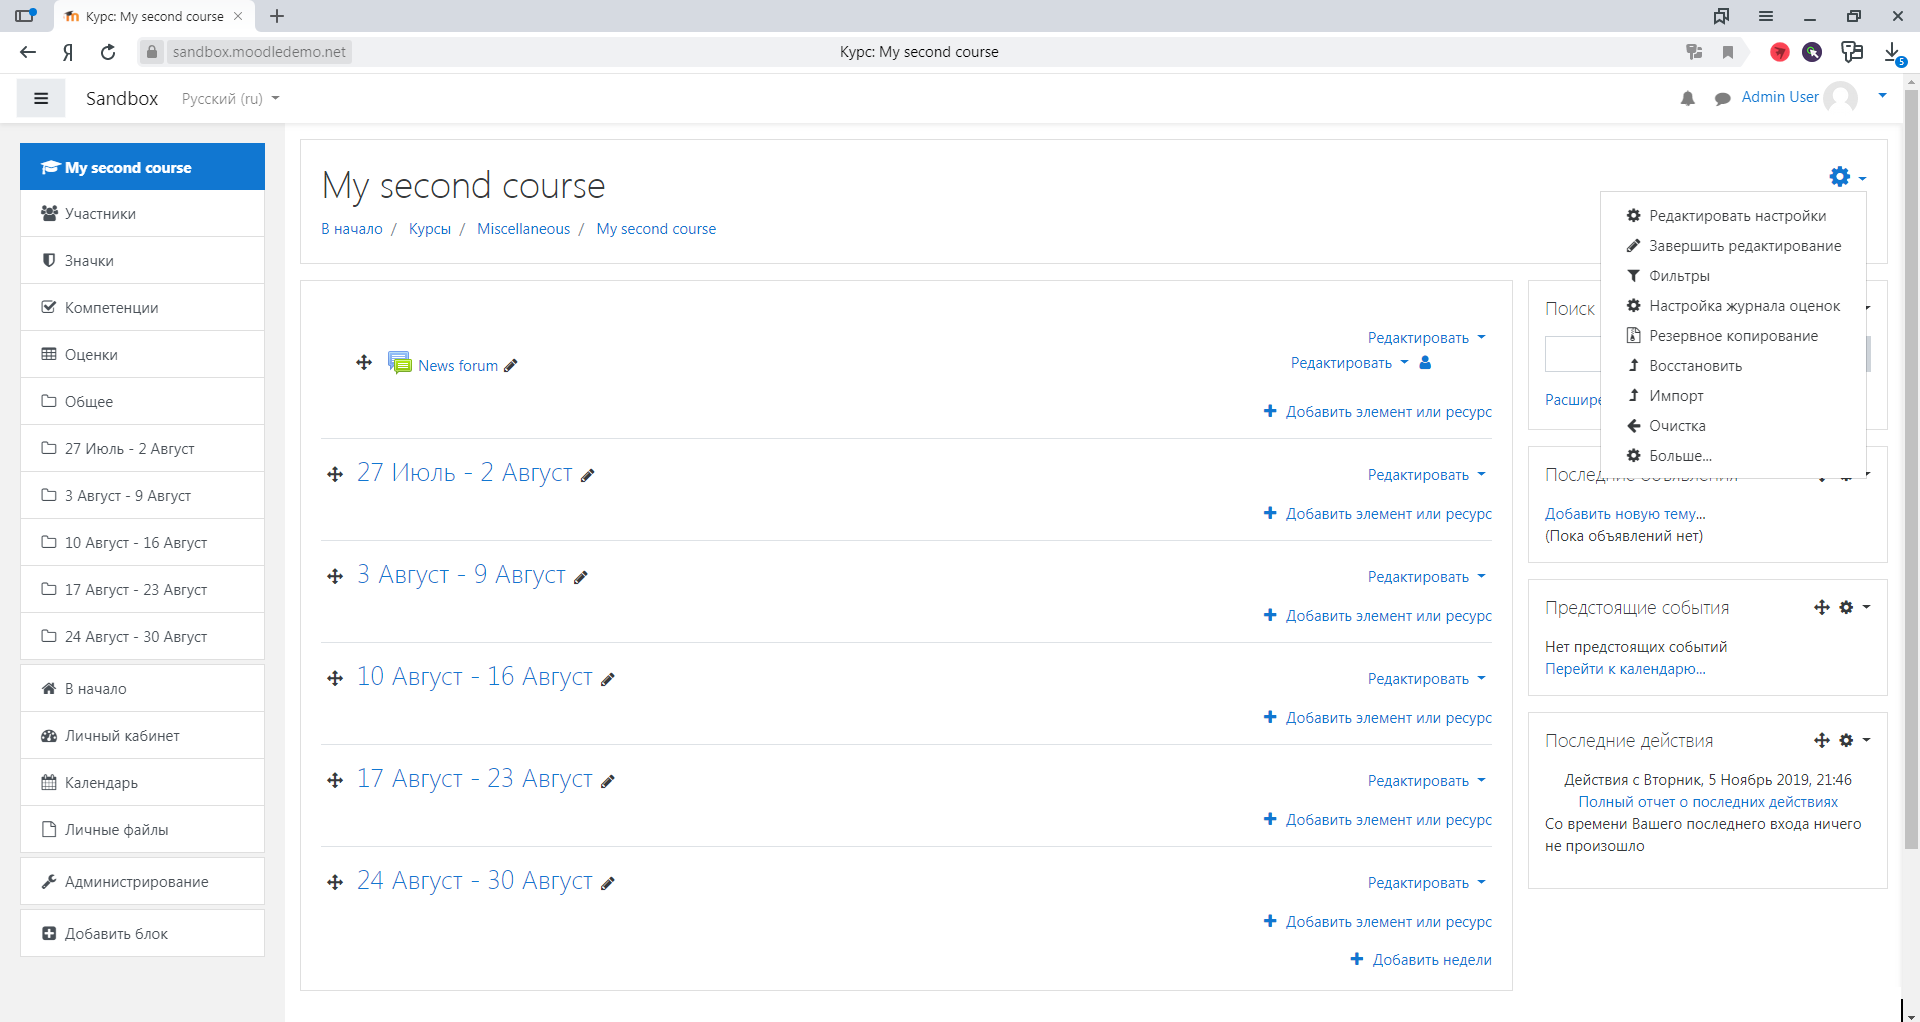
\includegraphics[width=0.9\linewidth]{picture/Moodle.png}
\caption{Интерфейс системы управления обучением Moodle}
\label{fig:moodle}
\end{figure}

Интерфейс системы (рисунок \ref{fig:moodle}) отражает ее административную направленность:
\begin{enumerate}[label=\arabic*]
\item Централизованное хранение методических материалов, лекций и заданий по дисциплинам.
\item Встроенный календарь, автоматически отображающий сроки сдачи контрольных работ, тестов и проектов, назначенных преподавателем.
\item Модули для загрузки выполненных заданий, ведения электронного журнала оценок и коммуникации с преподавательским составом.
\item Система генерирует цифровой след обучения и устанавливает глобальные цели, однако не предоставляет обучающемуся персональных средств для пошаговой декомпозиции этих задач, управления собственным ресурсом или проактивной борьбы с академической задолженностью. Платформа ориентирована на организацию процесса со стороны учебного заведения, а не студента.
\end{enumerate}

\subsection{Анализ подходов к разработке системы}

Для успешного решения выявленных проблем организации времени в академической среде недостаточно использовать традиционные алгоритмические методы. Эволюция систем искусственного интеллекта обусловила фундаментальный переход от парадигмы реактивных диалоговых интерфейсов к проактивным агентным рабочим процессам (Agentic Workflows). Разработка интеллектуального ассистента требует интеграции методов обработки естественного языка, дискретной оптимизации и проектирования гибридных интерфейсов. Ниже рассмотрены ключевые технологические подходы, применимые для реализации подобной системы.

% \stepcounter{subsubsection}
% \subsubsection*{\thesubsubsection\space Архитектурные парадигмы интеллектуального планирования}
\subsubsection{Архитектурные парадигмы интеллектуального планирования}

С точки зрения информатики, управление ресурсами и составление расписаний традиционно формулируются как задачи удовлетворения ограничений (Constraint Satisfaction Problems, CSP)~\cite{Rossi1999}. Несмотря на успехи больших языковых моделей (LLM), их архитектура делает прямое использование для решения сложных многомерных CSP-задач неэффективным. При попытке автономно сгенерировать оптимальное расписание с учетом множества ограничений, модели часто генерируют правдоподобные, но математически некорректные планы, что квалифицируется как «галлюцинации планирования».

Для преодоления этих ограничений применяется гибридный (нейросимволический) подход, известный как формализованное программирование на базе языковых моделей (LLM-Based Formalized Programming, LLMFP)~\cite{Hao2025}. В этой парадигме языковая модель не решает задачу расписания самостоятельно, а выполняет функцию интеллектуального транслятора. Модель анализирует естественный язык пользователя (например, описание учебной задачи), производит ее когнитивную декомпозицию и формирует набор структурированных параметров. Непосредственное размещение задач в календарной сетке и разрешение временных конфликтов делегируется строгой математической логике традиционных алгоритмов на стороне сервера. 

% \stepcounter{subsubsection}
% \subsubsection*{\thesubsubsection\space Управление знаниями и контекстом}
\subsubsection{Управление знаниями и контекстом}

Эффективный академический ассистент должен обладать доступом к контексту: учебным планам, методическим пособиям и истории активности обучающегося. Существует две фундаментальные стратегии обеспечения моделей этими данными: технология поисковой генерации (Retrieval-Augmented Generation, RAG)~\cite{Lewis2020} и прямая подача данных в модели с длинным контекстным окном (Long Context Window, LCW)~\cite{Liu2023}.

Подход RAG основан на фрагментации исходных документов, их векторизации и извлечении только семантически близких к запросу фрагментов. Это экономически эффективно, но при многоуровневых рассуждениях может приводить к потере глобальных связей. В свою очередь, LCW-модели способны одновременно анализировать весь объем информации, выявляя сложнейшие перекрестные зависимости без потери контекста. Оптимальным подходом к разработке признается гибридная стратегия, где RAG выступает в роли долгосрочной памяти для статических данных, а LCW применяется в качестве рабочей памяти для оперативного логического анализа.

% \stepcounter{subsubsection}
% \subsubsection*{\thesubsubsection\space Детерминированность взаимодействия и безопасность исполнения}
\subsubsection{Детерминированность взаимодействия и безопасность исполнения}

Интеграция языковой модели с программными интерфейсами (например, API календаря) требует, чтобы ответ агента был строго структурирован и гарантированно валиден, как правило, в формате JSON. Стохастическая природа нейросетей делает их склонными к синтаксическим ошибкам. В современной инженерии эта проблема решается через механизмы схема-ориентированного парсинга (Schema-Aligned Parsing) и нативные структурированные выводы (Structured Outputs)\cite{Rein2024}, которые принудительно ограничивают пространство генерации токенов, гарантируя совпадение результата с заданной структурой данных.

Наделение автономных систем доступом к личным данным переводит их в категорию активных агентов, что требует строгих мер безопасности. Для предотвращения нежелательных манипуляций с расписанием применяется архитектурный паттерн интеграции человека в контур управления (Human-in-the-Loop)~\cite{Holzinger2016}. Данный механизм контроля во время выполнения заставляет агента прервать работу, сгенерировать «черновик» решения и запросить одобрение у пользователя перед применением необратимого действия, например, созданием или удалением событий.

% \stepcounter{subsubsection}
% \subsubsection*{\thesubsubsection\space Проектирование гибридных пользовательских интерфейсов}
\subsubsection{Проектирование гибридных пользовательских интерфейсов}

Доминирующая парадигма взаимодействия через простой чат перекладывает когнитивную нагрузку на пользователя, заставляя его формулировать сложные запросы. Для достижения продуктивности концепция системы должна трансформироваться в агентный пользовательский интерфейс (Agentic UI)~\cite{Zhao2024} — гибридный формат, органично сочетающий понимание естественного языка с интерактивными графическими элементами.

Данный подход подразумевает использование управляемых форм для сбора намерений и инлайн-генерацию структур. Когда искусственный интеллект осуществляет декомпозицию курсового проекта, результат не выводится массивом текста, а визуализируется в виде редактируемых графических компонентов (например, шкал прогресса или карточек событий). Гибридный подход избавляет обучающегося от необходимости вести непрерывный диалог с машиной, предоставляя ассистенту роль архитектора, который предлагает оптимальные проекты расписания с возможностью их удобной ручной корректировки.

\subsection{Вывод}

В рамках данного раздела был проведен комплексный анализ предметной области, позволивший всесторонне охарактеризовать проблему организации времени в академической среде. Исследование психолого-педагогических аспектов выявило, что ключевым фактором возникновения прокрастинации является дефицит навыков саморегуляции при столкновении со слабоструктурированными долгосрочными задачами.

Критический обзор существующих программных аналогов и передовых архитектурных подходов показал перспективность интеграции языковых моделей (LLM) и детерминированных алгоритмов. Это позволяет автоматизировать рутину планирования, избегая при этом галлюцинаций в расписании.

На основании результатов проведенного анализа сформулированы первичные функциональные требования к разрабатываемому программному продукту. Для успешной компенсации когнитивных факторов прокрастинации интеллектуальный ассистент должен:
\begin{itemize}
    \item обеспечивать автоматизированную помощь в целеполагании и декомпозиции глобальных учебных проектов на атомарные шаги (спринты);
    \item реализовывать алгоритмическое планирование и расстановку приоритетов, эффективно распределяя временные ресурсы пользователя;
    \item осуществлять объективную оценку времени и динамическое разрешение конфликтов в календарной сетке;
    \item отслеживать расход времени в процессе работы над долгосрочной задачей, поддерживая фокус внимания через визуализацию прогресса и уведомления.
\end{itemize}

Сформулированный перечень концептуальных требований и выявленный вектор взаимодействия с пользователем являются базисом для перехода к следующему этапу исследования — детальному проектированию архитектуры системы, алгоритмов взаимодействия компонентов и составлению строгих технических спецификаций.